\documentclass{article}
\usepackage[utf8]{inputenc}
\usepackage{graphicx}
\usepackage{fullpage}


\begin{document}
\vspace{12pt}
\subsection{Problem Domain Model - Calculator}
\begin{figure}[h!]
    \centering
    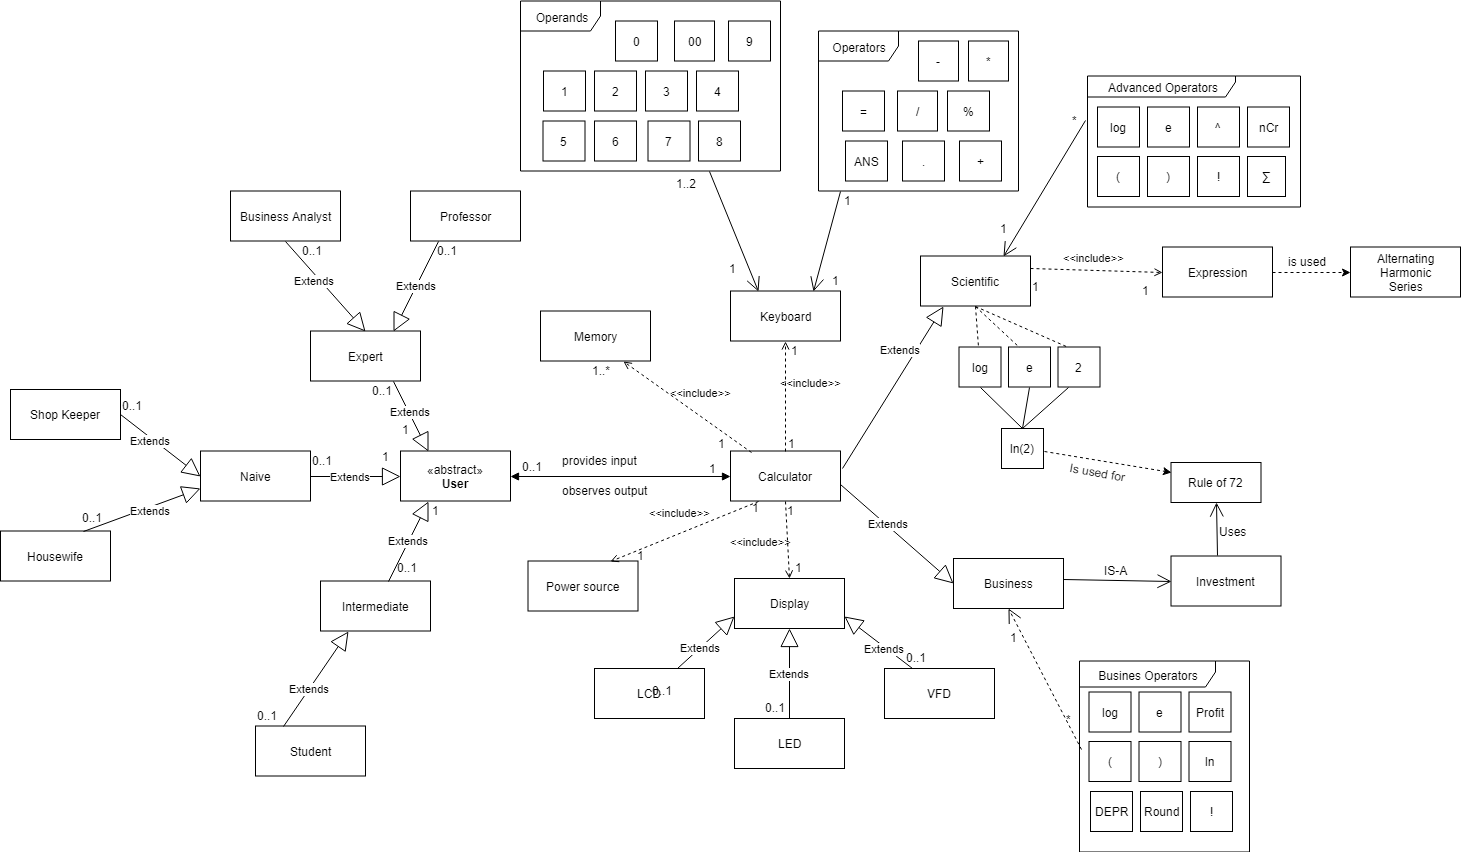
\includegraphics[angle=270,scale=0.37]{Problem_4.png}
\end{figure}
\newpage
\subsection{Description of relationship}
\begin{enumerate}
    \item User: Who uses the calculator.
    \begin{itemize}
        \item Expert User: A user who is using the calculator more often.
        \item Intermediate User: A user who is learning or have modrate use of a calculator.
        \item Naive User: A user who uses the calculator seldom. 
    \end{itemize}
    \item Calculator: Its an combination of components like Input/output devices, memory to perform basic computation and it requires power source. It's operated by a user.
    \item Display: A calculator must have a display either LCD(liquid crystal displays), LED(light emitting diode) or VFD(vacuum fluorescent displays).
    \item Memory: A calculator can not work without registers and memory.
    \item Power Source: A calculator requires power to work.
    \item Keyboard: A basic calculator requires a keyboard consisting of buttons which represents operands and operators.
    \item Operators: A frame of all the basic operators which includes both unary and binary operators. A single operator is needed to perform one basic operation.
    \item Operands: It consist of integers that a basic calculator has. one or two operands are needed depending on unary or binary operator.
    \item Scientific: A basic calculator is extended by the advanced scientific calculator which has few more complex operators.
    \item Expression: An expression is a collection of all the basic operations. A scientific calculator must have an expression.
    \item Advanced Operators: a frame that consist of all the advanced operators. We can use from 1 to n number of operators to be used in our expression.
    \item log - e - 2 : We use this collection of operators and operand to derive the value of $\ln(2)$.
    \item Rule of 72: The Rule of 72 is a quick, useful formula that is popularly used to estimate the number of years required to double the invested money at a given annual rate of return. \\
    $T \simeq \frac{\ln(2)}{\ln(1+\frac{r}{100})}$
    where: \\
    T = Time to double. \\
    r = Compounded interest rate per period.
    \item: Business: A Business calculator extends basic calculator and has some operators related to the business.
    \item Business Operator: It consist of various operators which are used in business.
    \item Investment: A business can be an Investment business which provides best solutions to the client to invest and earn more money. To calculate the approximated time we use the Rule of 72.
    \item Alternating Harmonic Series: We can compute the Alternating Harmonic Series. Its sum of $\frac{1}{n}$ where n starts from 1 to infinity and the sign alternates from positive to negative alternatively. \\
    $\sum_1^\infty{\frac{(-1)^{k+1}}{k}} = \ln(2) = 0.693..$ \\
    We can compute this value by the expression of the scientific calculator.
\end{enumerate}


\end{document}